\documentclass[border=3pt]{standalone}
% Preâmbulo compartilhado pelos diagramas TikZ da aula 9 de IHC (Princípios e Diretrizes)
\usepackage[T1]{fontenc}
\usepackage[utf8]{inputenc}
\usepackage{lmodern}
\usepackage{amsmath}
\usepackage{xcolor}
\usepackage{tikz}
\usetikzlibrary{arrows.meta,angles,quotes,decorations.pathmorphing,decorations.pathreplacing,calc,
                positioning,shapes.geometric,shapes.misc,backgrounds,fit,
                math}

% Paleta (mesma dos SVGs originais)
% Paleta da disciplina de IHC: acento roxo (#755099), da capa do livro.
% (o nome "dblue" é mantido para não alterar todos os diagramas)
\definecolor{dblue}{HTML}{755099}
\definecolor{dorange}{HTML}{B3541E}
\definecolor{dgreen}{HTML}{4A7C59}
\definecolor{dred}{HTML}{9C4B4B}
\definecolor{dcream}{HTML}{F4F1EA}
\definecolor{dshade}{HTML}{DDD7C9}

% Função gaussiana (não normalizada por padrão de escala visual)
\pgfmathdeclarefunction{gauss}{3}{%
  \pgfmathparse{1/(#3*sqrt(2*pi))*exp(-((#1-#2)^2)/(2*#3^2))}%
}

% Estilos comuns (prefixo d... para não colidir com chaves internas do pgf)
\tikzset{
  >={Stealth[length=2mm]},
  dguide/.style={gray!55, dashed, line width=0.4pt},
  daxis/.style={gray!60, line width=0.7pt, ->},
  dbody/.style={fill=black!3, draw=black!80, line width=1pt},
  dacc/.style={draw=dblue, line width=1pt},
  dlbl/.style={black!55, font=\small},
  dsub/.style={black!45, font=\footnotesize},
  dstate/.style={circle, draw=black!80, fill=dcream, line width=1pt,
                 minimum size=17mm, font=\large, inner sep=1pt},
  dobs/.style={circle, draw=black!80, fill=dshade, line width=1pt,
               minimum size=14mm, font=\large, inner sep=1pt},
  dbox/.style={rounded corners=2pt, draw=black!80, fill=dcream, line width=1pt,
               align=center, inner sep=6pt},
  dop/.style={circle, draw=black!80, fill=white, line width=1pt,
              minimum size=6mm, inner sep=0pt, font=\small},
  dtrans/.style={->, dblue, line width=1pt},
  dmeas/.style={->, dorange, line width=1pt},
  dcurve/.style={line width=1pt, dblue},
  dcurveb/.style={line width=1.4pt, dorange},
}

\begin{document}
\hyphenpenalty=10000 \exhyphenpenalty=10000 \tolerance=9999 \emergencystretch=3em
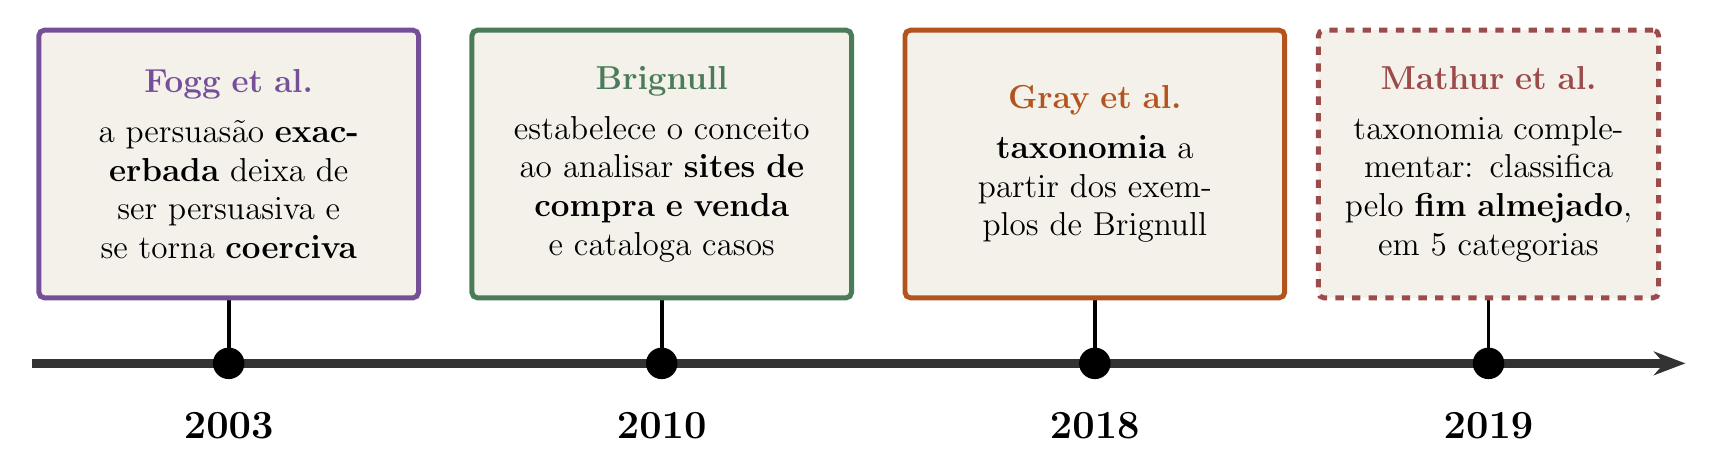
\begin{tikzpicture}[x=1cm,y=1cm]
\tikzset{k/.style={dbox, text width=4.4cm, minimum height=3.4cm, font=\large, line width=1.8pt}}
\draw[line width=3pt, draw=black!80, -{Stealth[length=4mm]}] (0,2.3) -- (21.0,2.3);
\foreach \x/\a in {2.5/2003, 8.0/2010, 13.5/2018, 18.5/2019} {
  \fill[black] (\x,2.3) circle (0.2);
  \node[font=\Large\bfseries, anchor=north] at (\x,1.8) {\a};
  \draw[line width=1.4pt, black] (\x,2.5) -- (\x,3.1);}
\node[k, draw=dblue, anchor=south] at (2.5,3.1) {\textbf{\textcolor{dblue}{Fogg et al.}}\\[4pt] a persuasão \textbf{exacerbada} deixa de ser persuasiva e se torna \textbf{coerciva}};
\node[k, draw=dgreen, anchor=south] at (8.0,3.1) {\textbf{\textcolor{dgreen}{Brignull}}\\[4pt] estabelece o conceito ao analisar \textbf{sites de compra e venda} e cataloga casos};
\node[k, draw=dorange, anchor=south] at (13.5,3.1) {\textbf{\textcolor{dorange}{Gray et al.}}\\[4pt] \textbf{taxonomia} a partir dos exemplos de Brignull};
\node[k, draw=dred, dashed, anchor=south, text width=3.9cm] at (18.5,3.1) {\textbf{\textcolor{dred}{Mathur et al.}}\\[4pt] taxonomia complementar: classifica pelo \textbf{fim almejado}, em 5 categorias};
\end{tikzpicture}
\end{document}
